\section{Aufbau}
\label{sec:Aufbau}
Der Aufbau der Wärmepumpe ist in \autoref{fig:Wärmepumpe_durch} zur Messung der gesuchten Kenngrößen dargestellt.
Sie besteht aus zwei Reservoiren, in denen sich Wasser befindet, welches von Rührmotoren durchrührt wird. 
Das ist wichtig, damit das Wasser eine homogene Temperatur besitzt und die zwei digitalen Thermometer, die sich in den Reservoiren befinden, die Temperatur des gesamten Wasser messen.
Die Teile sind alle verbunden mit einer Kupferschlange.
Das Wasser verdampft in Reservoir 2 und entzieht dem somit die Verdampfungswärme $L$.
Es ist somit das wärmeangebende, kältere Reservoir.
Es folgt eine Steuerungsvorrichtung, die gewährleistet, dass flüssige Überreste zerstört werden, sodass nur Dampf vorhanden ist.
Anschließend durchläuft der Dampf den Kompressor und wird dort adiabatisch komprimiert und somit stark erhitzt.
Im Reservoir 1 verflüssigt es sich, aufgrund der Druckerhöhung.
Währenddessen gibt das Wasser die Kondensationswärme $L$ an das Reservoir und erhitzt es.
Anschließend wird der Druck $p_b$ an dem Barometer abgelesen. 
Anschließend fließt die Flüssigkeit durch einen Reiniger, der die Flüssigkeit von Gasresten trennt, damit im folgenden das Drosselventil nicht beschädigt wird.
Nach dem Drosselventil wird der Druck $p_a$ gemessen und die Flüssigkeit gelangt ins Reservoir 2.
Außerdem ist der Kompressor an  ein Wattmeter angeschlossen, was dessen Leistung misst.
\begin{figure}[H]
    \centering
    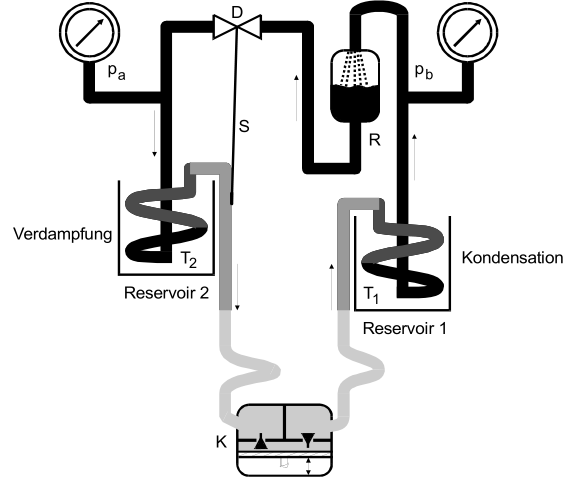
\includegraphics[width=0.6\textwidth]{build/Abb1.png}
    \caption{Schematische Darstellung der kompletten Messapparatur \cite[197]{V206}.}
    \label{fig:Wärmepumpe_durch}
\end{figure}
\section{Durchführung}
\label{sec:Durchführung}
